\documentclass[12pt]{article}
\usepackage{amsmath}
\usepackage{amssymb}
\usepackage{listings}
\usepackage{framed}
\usepackage{graphicx}
\usepackage{algorithm}
\usepackage{algorithmicx}
\usepackage{algpseudocode}

\author{Sean White, Kierstyn Brandt, Rostik Mertz, Norman Tang}
\title{CSCI 432 - Assignment G5}

\begin{document}
\maketitle

\noindent
\textbf{Question A:} For the algorithm in 16.12 (Find the Longest Nondecreasing Subsequence), what is the loop invariant? Note: be sure to fully justify. \smallskip

A loop invariant is a condition in a loop that is true both before and after an iteration of the loop. It may break anywhere during the loop, but as long as it is true by the end of that iteration these requirements are still met. For the Longest Nondecreasing Subsequence algorithm shown in 16.12 of \textit{Elements of Programming Interviews} let our loop invariant $L$ be that the vector $max\_length$ is populated with the maximum nondecreasing subsequences of $A$ ending at index $i - 1$. 

At the start of the loop $i$ is equal to 1 and $max\_length$ is initialized with length $= \|A\|$ and each element set to 1. The maximum possible length of any sequence only involving the $0^{th}$ element is 1 as nothing comes before it, therefore $L$ holds true. Now assume $L$ always holds true at the beginning of iteration $i$. This means that $max\_length$ holds the length of the nondecreasing subsequences of $A$ ending at index $i - 1$. The algorithm now runs through the second for loop calulating the maximum nondecreasing subsequence up to index $i$ and stores it in $max\_length$. So at the start of iteration $k = i + 1$, $max\_length$ holds maximum nondecreasing subsequences of $A$ ending at index $k - 1 = i$, so $L$ holds true at the $i + 1$ iteration as well.

At the termination of the loop we will have iterated through all the elements of $A$ and the calculated max nondecreasing subsequences have been stored in $max\_length$. This means that $max\_length$ holds values for sequences in $A$ up to $i$ which implies it has up to $i-1$ as well. Therefore, our $L$ holds at the beginning, end, and termination of the loop and counts as a valid loop invariant.


\pagebreak
\noindent
\textbf{Question B:} Add one source and one sink vertex ($s$ and $t$, respectively) to Figure 1. Connect $s$ to three vertices, and connect two different vertices to $t$. Add direction and weights to all edges so that the maximum flow / minimum cut of the flow network has value five (5). Annotate the edges clearly so that the max flow is shown, and draw a ‘blob’ (or, a topological disk) that shows what vertices are in S for the minimum cut. \smallskip

\bigskip
\noindent
\textbf{Question C:} Consider the graph in Figure 1. Answer the following questions regarding this graph.\smallskip

\smallskip
\noindent
(a) What is the Euler characteristic of the graph?\smallskip

|V| - E = Euler Characteristic.
-8 is the Euler Characteristic.

\smallskip
\noindent
(b) What is the graph genus? (minimum number of handles necessary to draw the graph without crossing)?\smallskip

The minimum number of handles is one, which gives us a 1-hole torus mapping.

	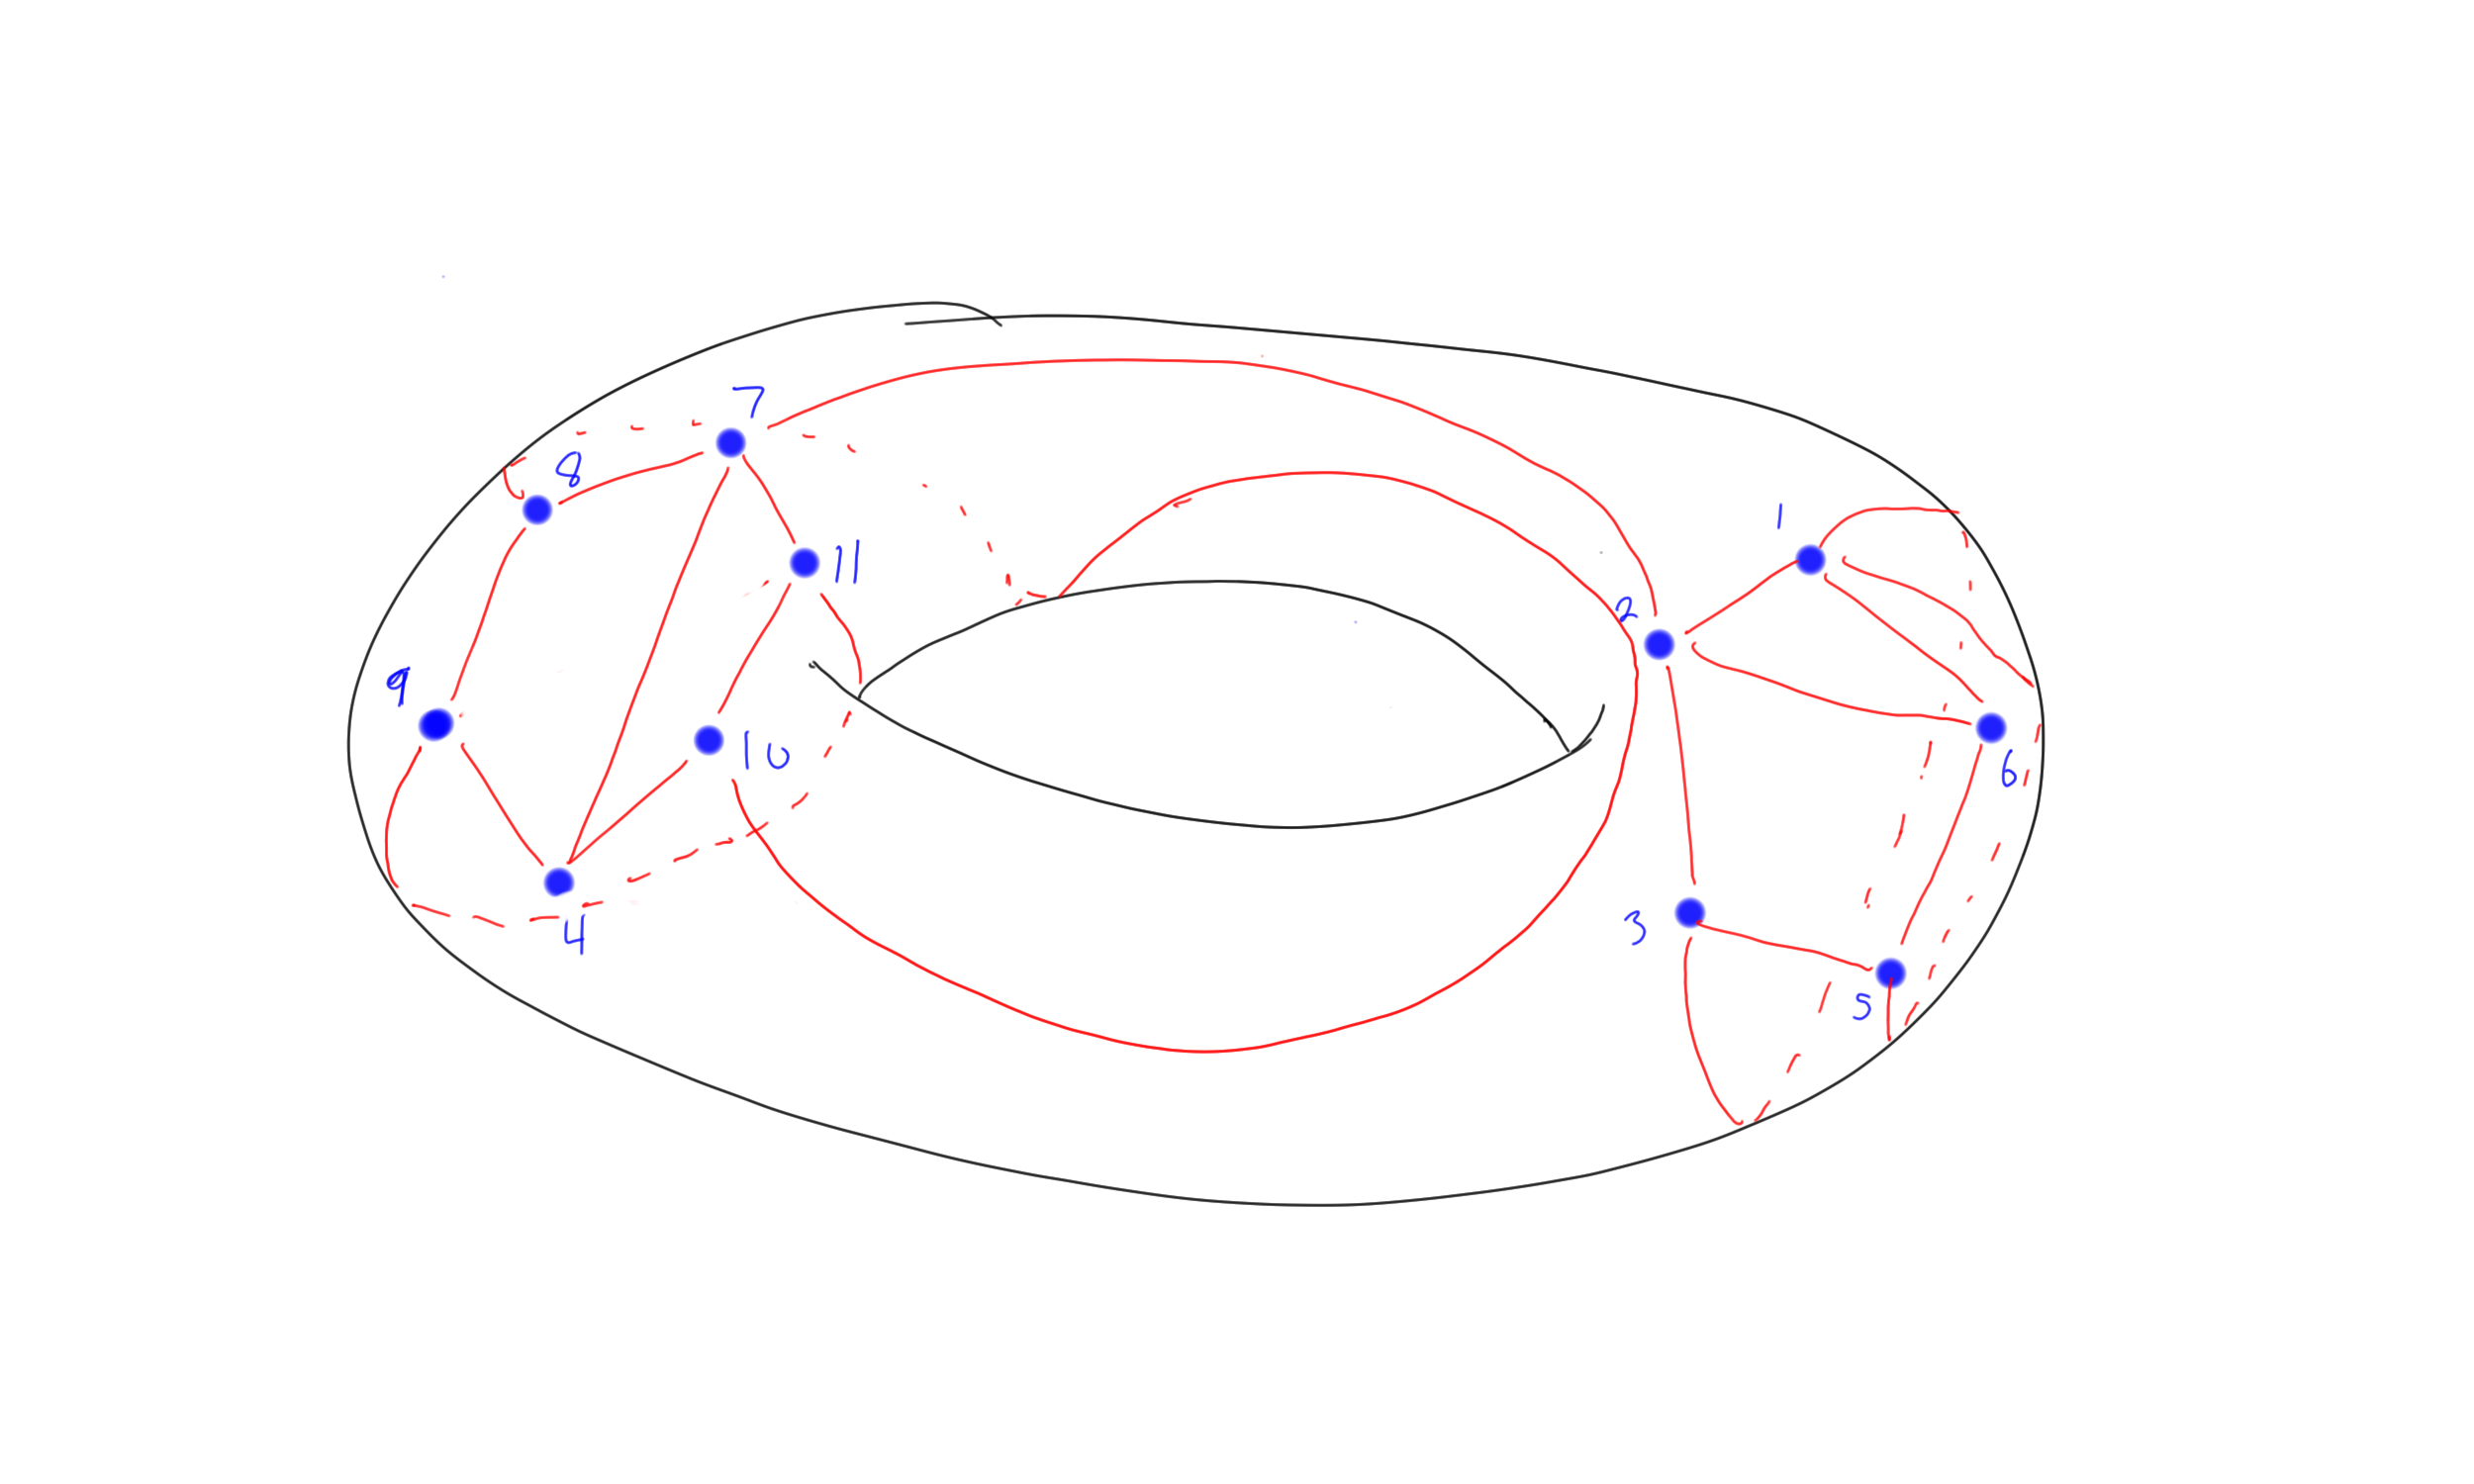
\includegraphics[width=\linewidth]{GraphTorus}


\smallskip
\noindent
(c) Is an Eulerian tour possible?\smallskip

No it is not, we do not have exactly 2 or no nodes with odd degrees. \smallskip

\newpage
\noindent
(d) Is a Hamiltonian path possible?\smallskip

Yes. The path the is as follows: $V_1, V_3, V_5, V_6, V_2, V_7, V_8, V_9, V_4, V_10, and V_11$. \smallskip

\smallskip
\noindent
(e) What is the size of the largest clique?\smallskip

It is: $V_1, V_2, V_3, V_5, and V_6$


\end{document}